\appendix

\chapter*{Une annexe}

\section*{Productions (code, logiciel)}

\subsection*{Corpus}

\subsubsection*{\textit{CREMMA Early Modern Books}}

Ce corpus avait pour objectif d'évaluer la capacité des modèles d'OCR pour le français de s'adapter à des oeuvres latines, à travers d'échantillons d'une dizaine de pages. 

\begin{itemize}
    \item Dépôt de code: \url{https://github.com/HTR-United/cremma-16-17-print}
    \item \cite{Clerice_CREMMA_16_18_Prints_2021}
\end{itemize}

\subsection*{Logiciels}

\subsubsection*{OCR Sycophant}

Logiciel d'analyse de ressources plein texte pour évaluer sommairement la qualité de l'OCR à base d'apprentissage de N-Grams.

\begin{itemize}
    \item Dépôt de code: \url{https://github.com/PonteIneptique/OCR-Sycophant}
    \item \cite{Clerice_OCR_Sycophant_2021}
\end{itemize}

\subsubsection*{Pyrrha}

Application pour la post-correction d'annotations linguistiques (lemmatisation, annotations morpho-syntaxique).

\begin{itemize}
    \item Dépôt de code: \url{https://github.com/hipster-philology/pyrrha}
    \item \cite{Clerice_Pyrrha_2021}
\end{itemize}

\section*{Exemples de test}[h]

\begin{figure}
\centering
\begin{adjustbox}{width=.9\linewidth}
\begin{lstlisting}[breaklines=false,columns=fullflexible,keepspaces]
+-----------------------------------------+---------+-------------+-----------------------------+
|                Identifier               |  Words  |    Nodes    |         Failed Tests        |
+-----------------------------------------+---------+-------------+-----------------------------+
|   dlt000123.dlt001.digilibLT-lat1.xml   |    0    |             |             All             |
+-----------------------------------------+---------+-------------+-----------------------------+
|  dlt000386.dlt000386.digilibLT-lat1.xml |  46,141 |    11;269   |                             |
+-----------------------------------------+---------+-------------+-----------------------------+
|  dlt000493.dlt000493.digilibLT-lat1.xml |   310   |      3      |                             |
+-----------------------------------------+---------+-------------+-----------------------------+
|    phi1257.phi001.digilibLT-lat1.xml    |  3,390  |    5;225    |                             |
+-----------------------------------------+---------+-------------+-----------------------------+
|   stoa0365.stoa002.digilibLT-lat1.xml   |  13,155 |   133;139   |                             |
+-----------------------------------------+---------+-------------+-----------------------------+
|    tlg4096.tlg001.digilibLT-lat1.xml    |    0    |             |    Passage level parsing    |
|                                         |         |             | Unique nodes found by XPath |
|                                         |         |             |       Empty References      |
|                                         |         |             |        Word Counting        |
+-----------------------------------------+---------+-------------+-----------------------------+

Duplicate nodes found:
	stoa0058.stoa001.digilibLT-lat1.xml	1, 2, 3, 4, 5, 6, 7, 8, I, II, III, IV, V, VI, VII, VIII
	stoa0357b.stoa001.digilibLT-lat1.xml	1, 12, 2, 24, 4, 5, 8, 9

Forbidden characters found:
	stoa0357d.stoa001.digilibLT-lat1.xml	'<386-387>', '<397-399>', '546-547'

DTD errors found:
	dlt000123.dlt001.digilibLT-lat1.xml	 fatal: The markup in the document following the 
	root element must be well-formed. [In (L216 C2)]
	stoa0167.stoa002.digilibLT-lat1.xml	 error: attribute "unit" not allowed here [In (L35 C132); 
	(L37 C159); (L38 C172)],  error: element "cRefPattern" not allowed here 
	[In (L37 C159); (L38 C172)]

>>> End of the test !

+----------------------+-----------+
|   HookTestResults    |           |
+----------------------+-----------+
|     Total Texts      |    216    |
+----------------------+-----------+
|    Passing Texts     |    103    |
+----------------------+-----------+
|    Metadata Files    |    348    |
+----------------------+-----------+
|   Passing Metadata   |    348    |
+----------------------+-----------+
|       Coverage       |   91.91   |
+----------------------+-----------+
| Total Citation Units |   51,212  |
+----------------------+-----------+
|     Total Words      | 2,755,504 |
+----------------------+-----------+
|     Words in LAT     | 2,754,128 |
+----------------------+-----------+
|     Words in GRC     |   1,376   |
+----------------------+-----------+
\end{lstlisting}
\end{adjustbox}
\caption{Exemple de résultats (tronqués) de HookTest sur le corpus DigilibLT.}
\label{fig:annx:digiliblt-hooktest}
\end{figure}

\section*{Résultats de lemmatiseurs}


\begin{table}[h]

\resizebox{\textwidth}{!}{%
\begin{tabular}{@{}l|llll||l|llll@{}}
 \toprule
 target            & precision & recall & f1-score & support &  target            & precision & recall & f1-score & support\\ \midrule
 Adj-N/A-Dep         & 0.90      & 0.87   & 0.88     & 61      & Par-Fut-Act       & 0.89      & 0.89   & 0.89     & 214     \\ 
 Adj-N/A-Pass        & 0.96      & 0.96   & 0.96     & 736     & Par-Fut-Dep       & 0.80      & 0.86   & 0.83     & 14      \\ 
 Adj-N/A-SemDep      & 1.00      & 0.67   & 0.80     & 3       & Par-Fut-SemDep    & 0.00      & 0.00   & 0.00     & 1       \\ 
 Ger-N/A-Act         & 0.91      & 0.90   & 0.91     & 273     & Par-Perf-Act      & 0.00      & 0.00   & 0.00     & 1       \\ 
 Ger-N/A-Dep         & 0.89      & 0.94   & 0.91     & 67      & Par-Perf-Dep      & 0.69      & 0.76   & 0.72     & 363     \\ 
 Ger-N/A-SemDep      & 1.00      & 1.00   & 1.00     & 1       & Par-Perf-Pass     & 0.74      & 0.84   & 0.79     & 2927    \\ 
 Imp-Fut-Act       & 0.97      & 0.96   & 0.96     & 142     & Par-Perf-SemDep   & 0.69      & 0.48   & 0.56     & 23      \\ 
 Imp-Fut-Dep       & 1.00      & 0.50   & 0.67     & 4       & Par-Pres-Act      & 0.94      & 0.96   & 0.95     & 1210    \\ 
 Imp-Pres-Act      & 0.97      & 0.95   & 0.96     & 805     & Par-Pres-Dep      & 0.96      & 0.96   & 0.96     & 188     \\ 
 Imp-Pres-Dep      & 0.91      & 0.91   & 0.91     & 54      & Par-Pres-SemDep   & 0.80      & 0.80   & 0.80     & 5       \\ 
 Imp-Pres-Pass     & 0.00      & 0.00   & 0.00     & 1       & Sub-Fut-Act       & 1.00      & 1.00   & 1.00     & 28      \\ 
 Imp-Pres-SemDep   & 1.00      & 1.00   & 1.00     & 5       & Sub-Fut-Dep       & 0.00      & 0.00   & 0.00     & 1       \\ 
 Ind-Fut-Act       & 0.95      & 0.90   & 0.92     & 1581    & Sub-Fut-Pass      & 0.00      & 0.00   & 0.00     & 10      \\ 
 Ind-Fut-Dep       & 0.90      & 0.90   & 0.90     & 108     & Sub-Impa-Act      & 1.00      & 1.00   & 1.00     & 1541    \\ 
 Ind-Fut-Pass      & 0.95      & 0.75   & 0.84     & 144     & Sub-Impa-Dep      & 0.99      & 0.99   & 0.99     & 136     \\ 
 Ind-Fut-SemDep    & 1.00      & 1.00   & 1.00     & 5       & Sub-Impa-Pass     & 0.99      & 0.99   & 0.99     & 308     \\ 
 Ind-Impa-Act      & 1.00      & 1.00   & 1.00     & 1336    & Sub-Impa-SemDep   & 1.00      & 1.00   & 1.00     & 17      \\ 
 Ind-Impa-Dep      & 0.97      & 0.98   & 0.98     & 113     & Sub-Perf-Act      & 0.80      & 0.95   & 0.87     & 459     \\ 
 Ind-Impa-Pass     & 0.99      & 0.99   & 0.99     & 235     & Sub-Perf-Dep      & 0.53      & 0.44   & 0.48     & 18      \\ 
 Ind-Impa-SemDep   & 1.00      & 1.00   & 1.00     & 40      & Sub-Perf-Pass     & 0.25      & 0.15   & 0.19     & 92      \\ 
 Ind-Perf-Act      & 0.97      & 0.97   & 0.97     & 4056    & Sub-Perf-SemDep   & 0.00      & 0.00   & 0.00     & 2       \\ 
 Ind-Perf-Dep      & 0.63      & 0.59   & 0.61     & 208     & Sub-PeriPerf-Pass & 0.00      & 0.00   & 0.00     & 3       \\ 
 Ind-Perf-Pass     & 0.58      & 0.55   & 0.57     & 827     & Sub-PeriPqp-Dep   & 0.00      & 0.00   & 0.00     & 1       \\ 
 Ind-Perf-SemDep   & 0.56      & 0.74   & 0.64     & 19      & Sub-PeriPqp-Pass  & 0.00      & 0.00   & 0.00     & 4       \\ 
 Ind-PeriFut-Pass  & 0.00      & 0.00   & 0.00     & 2       & Sub-Pqp-Act       & 1.00      & 1.00   & 1.00     & 569     \\ 
 Ind-PeriPerf-Pass & 0.00      & 0.00   & 0.00     & 5       & Sub-Pqp-Dep       & 0.29      & 0.26   & 0.28     & 19      \\ 
 Ind-PeriPqp-Dep   & 0.00      & 0.00   & 0.00     & 2       & Sub-Pqp-Pass      & 0.42      & 0.22   & 0.29     & 68      \\ 
 Ind-PeriPqp-Pass  & 0.00      & 0.00   & 0.00     & 4       & Sub-Pqp-SemDep    & 0.00      & 0.00   & 0.00     & 5       \\ 
 Ind-Pqp-Act       & 1.00      & 1.00   & 1.00     & 639     & Sub-Pres-Act      & 0.97      & 0.97   & 0.97     & 2617    \\ 
 Ind-Pqp-Dep       & 0.00      & 0.00   & 0.00     & 10      & Sub-Pres-Dep      & 0.95      & 0.93   & 0.94     & 197     \\ 
 Ind-Pqp-Pass      & 0.42      & 0.11   & 0.18     & 90      & Sub-Pres-Pass     & 0.98      & 0.94   & 0.96     & 332     \\ 
 Ind-Pqp-SemDep    & 0.33      & 0.40   & 0.36     & 5       & Sub-Pres-SemDep   & 0.96      & 0.96   & 0.96     & 25      \\ 
 Ind-Pres-Act      & 0.98      & 0.98   & 0.98     & 8453    & SupUm-N/A-Act       & 0.92      & 0.65   & 0.76     & 17      \\ 
 Ind-Pres-Dep      & 0.97      & 0.98   & 0.97     & 689     & SupU-N/A-Act        & 0.77      & 0.67   & 0.71     & 15      \\ 
 Ind-Pres-Pass     & 0.99      & 0.98   & 0.98     & 963     & SupU-N/A-Dep        & 0.83      & 0.71   & 0.77     & 7       \\ 
 Ind-Pres-SemDep   & 1.00      & 1.00   & 1.00     & 109     & N/A               & 1.00      & 1.00   & 1.00     & 133503  \\ 
 Inf-Fut-Act       & 0.86      & 0.95   & 0.90     & 194     \\ 
 Inf-Fut-Dep       & 0.92      & 0.75   & 0.83     & 16      \\ 
 Inf-Fut-Pass      & 0.00      & 0.00   & 0.00     & 1       \\ 
 Inf-Fut-SemDep    & 0.67      & 1.00   & 0.80     & 2       \\ 
 Inf-Perf-Act      & 1.00      & 1.00   & 1.00     & 586     \\ 
 Inf-Perf-Dep      & 0.49      & 0.66   & 0.56     & 32      \\ 
 Inf-Perf-Pass     & 0.59      & 0.48   & 0.53     & 368     \\ 
 Inf-Perf-SemDep   & 0.57      & 1.00   & 0.73     & 4       \\ 
 Inf-PeriFut-Act   & 0.00      & 0.00   & 0.00     & 9       \\ 
 Inf-PeriPqp-Pass  & 0.00      & 0.00   & 0.00     & 3       \\ 
 Inf-Pres-Act      & 0.99      & 1.00   & 0.99     & 3720    \\ 
 Inf-Pres-Dep      & 0.98      & 0.96   & 0.97     & 428     \\ 
 Inf-Pres-Pass     & 0.96      & 0.97   & 0.97     & 854     \\ 
 Inf-Pres-SemDep   & 1.00      & 1.00   & 1.00     & 16      \\ 
 avg / total       & 0.67      & 0.66   & 0.66     & 172968  \\ \bottomrule
\end{tabular}}
\caption{Résultat sur les données brutes du LASLA pour les annotations verbales hors personne}
\label{table:lasla:verb-scores}
\end{table}


\begin{table}[h]
\begin{tabular}{lrrrrrrrr}
\hline
               &     0.01 &     0.05 &      0.1 &      0.2 &      0.25 &      0.3 &      0.4 &      0.5 \\
 Caesar        &   536    &  3224    &   6784   &  13525   &  17071    &  20843   &  28460   &  35607   \\
 Cato          &   172    &   977    &   1795   &   4107   &   4930    &   5649   &   7098   &   8601   \\
 Catullus      &   160    &   611    &   1084   &   2225   &   2825    &   3271   &   4254   &   4899   \\
 Cicero        &  5067    & 25296    &  47651   &  90787   & 111373    & 130462   & 170087   & 209291   \\
 Curtius       &   404    &  2901    &   5977   &  12330   &  15589    &  18233   &  24140   &  30352   \\
 Hirtius       &    59    &   313    &    597   &   1251   &   1525    &   1851   &   2369   &   2960   \\
 Horatius      &   257    &  2046    &   4084   &   8016   &  10016    &  12078   &  15874   &  19855   \\
 Juvenalis     &   304    &   989    &   1921   &   4126   &   5175    &   6267   &   8100   &  10586   \\
 Lucretius     &   614    &  2664    &   4947   &   9255   &  11506    &  13828   &  18419   &  23012   \\
 Ovidius       &   799    &  4525    &   9158   &  17711   &  22023    &  26503   &  35741   &  44389   \\
 Persius       &    41    &   113    &    331   &    751   &    949    &   1128   &   1522   &   2038   \\
 Petronius     &   411    &  1595    &   3203   &   5667   &   6513    &   7632   &  10073   &  12598   \\
 Plautus       &   827    &  3469    &   6426   &  11636   &  13760    &  16390   &  21760   &  26340   \\
 Plinius       &   789    &  3813    &   7506   &  15135   &  19232    &  23315   &  30850   &  38437   \\
 Propertius    &   230    &  1291    &   2660   &   4962   &   6202    &   7304   &   9526   &  11912   \\
 PseudoCaesar1 &    72    &   460    &   1028   &   2371   &   2908    &   3590   &   4822   &   5954   \\
 PseudoCaesar2 &   129    &   485    &    930   &   1704   &   2146    &   2663   &   3605   &   4613   \\
 PseudoCaesar3 &     5    &   106    &    317   &    588   &    720    &    863   &   1257   &   1859   \\
 Sallustius    &   347    &  1765    &   3204   &   6407   &   7980    &   9609   &  12966   &  16563   \\
 Seneca        &  3374    & 16028    &  30275   &  58539   &  72262    &  84821   & 113123   & 140158   \\
 Tacitus       &  1413    &  7702    &  14826   &  29697   &  36707    &  44223   &  58931   &  73242   \\
 Tibullus      &    87    &   564    &   1123   &   2277   &   2813    &   3358   &   4294   &   5577   \\
 Vergilius     &   714    &  3745    &   7567   &  15307   &  19267    &  23359   &  31348   &  39075   \\
 Total         & 16811    & 84682    & 163394   & 318374   & 393492    & 467240   & 618619   & 767918   \\
\hline
\end{tabular}
\caption{Nombre de tokens par auteur en fonction du pourcentage de coupe }
\label{table:lasla:extensibilite}
\end{table}


\begin{table}[h]
\centering
\begin{tabular}{l|lll|lll}
\toprule
 File         & Tokens &      &      & Chunks &     &      \\
              & Train  & Dev  & Test & Train  & Dev & Test \\ \midrule
 Petron, Sa   & 1955   & 176  & 402  & 136    & 14  & 28   \\
 Ov, Fasti, 1 & 2251   & 208  & 455  & 136    & 14  & 28   \\
 Ov, Fasti, 2 & 1901   & 186  & 445  & 136    & 14  & 28   \\
 Ov, Fasti, 3 & 2225   & 154  & 439  & 136    & 14  & 28   \\
 Tac, Hist, 1 & 281    & 72   & 51   & 13     & 2   & 3    \\
 Tac, Hist, 2 & 251    & 70   & 88   & 13     & 2   & 3    \\
 Tac, Hist, 3 & 269    & 40   & 57   & 13     & 2   & 3    \\
 Tac, Hist, 4 & 592    & 30   & 95   & 13     & 2   & 3    \\
 Tac, Hist, 5 & 516    & 126  & 144  & 13     & 2   & 3    \\
 Caes, BG, 1  & 146    & 26   & 54   & 4      & 1   & 1    \\
 Caes, BG, 2  & 110    & 63   & 23   & 4      & 1   & 1    \\
 Caes, BG, 3  & 76     & 32   & 19   & 4      & 1   & 1    \\
 Caes, BG, 4  & 99     & 32   & 30   & 4      & 1   & 1    \\
 Caes, BG, 5  & 73     & 10   & 16   & 4      & 1   & 1    \\
 Caes, BG, 6  & 132    & 7    & 8    & 4      & 1   & 1    \\
 Caes, BG, 7  & 69     & 15   & 22   & 4      & 1   & 1    \\
 Cic, Cat, 1  & 705    & 90   & 157  & 35     & 4   & 7    \\
 Cic, Cat, 2  & 819    & 101  & 138  & 35     & 4   & 7    \\
 Cic, Cat, 3  & 1014   & 149  & 102  & 35     & 4   & 7    \\
 Cic, Cat, 4  & 933    & 111  & 192  & 35     & 4   & 7    \\
 Propert, 1   & 952    & 113  & 250  & 56     & 6   & 12   \\
 Propert, 2   & 1002   & 75   & 314  & 56     & 6   & 12   \\
 Propert, 3   & 875    & 67   & 258  & 56     & 6   & 12   \\
 Propert, 4   & 1029   & 88   & 149  & 56     & 6   & 12   \\
 Sal, Catil   & 7389   & 617  & 1562 & 336    & 34  & 67   \\
 Ver, Aen, 1  & 27     & 29   & 7    & 2      & 1   & 1    \\
 Ver, Aen, 2  & 24     & 29   & 27   & 2      & 1   & 1    \\
 Ver, Aen, 3  & 42     & 39   & 24   & 2      & 1   & 1    \\
 Ver, Aen, 4  & 35     & 9    & 56   & 2      & 1   & 1    \\
 Ver, Aen, 5  & 41     & 33   & 20   & 2      & 1   & 1    \\
 Ver, Aen, 6  & 30     & 49   & 22   & 2      & 1   & 1    \\
 Ver, Aen, 7  & 31     & 25   & 6    & 2      & 1   & 1    \\
 Ver, Aen, 8  & 43     & 19   & 30   & 2      & 1   & 1    \\
 Ver, Aen, 9  & 19     & 35   & 15   & 2      & 1   & 1    \\
 Ver, Aen, 10 & 47     & 44   & 3    & 2      & 1   & 1    \\
 Ver, Aen, 11 & 33     & 14   & 31   & 2      & 1   & 1    \\
 Ver, Aen, 12 & 45     & 15   & 7    & 2      & 1   & 1    \\ \midrule
 Total        & 26081  & 2998 & 5718 & 1361   & 159 & 289  \\ \bottomrule
\hline
\end{tabular}
\caption{Répartition par oeuvres du nombres de séquences et de tokens dans les corpus d'entraînement PerseusUD en LASLA}
\label{table:lasla:perseus-ud}
\end{table}


\begin{table}[]
    \centering
    \resizebox{!}{.35\paperheight}{%
    \begin{tabular}{lrrrrrrrrr}
    \toprule
    Priapée &  lemma &   Deg &  Numb &  Person &  Mood\_Tense\_Voice &  Case &  Gend &   pos &  Taille \\
    \midrule
    1  &  0.920 & 0.980 & 0.940 &   0.980 &             0.940 & 0.860 & 0.860 & 0.920 &    51 \\
    2  &  0.964 & 1.000 & 0.964 &   1.000 &             0.964 & 0.945 & 0.891 & 1.000 &    56 \\
    3  &  0.956 & 0.971 & 0.941 &   1.000 &             1.000 & 0.897 & 0.868 & 0.941 &    69 \\
    4  &  0.947 & 1.000 & 1.000 &   1.000 &             1.000 & 0.789 & 1.000 & 1.000 &    20 \\
    5  &  0.885 & 1.000 & 0.962 &   1.000 &             0.962 & 0.846 & 0.923 & 1.000 &    27 \\
    6  &  0.935 & 1.000 & 0.968 &   1.000 &             1.000 & 0.903 & 0.935 & 1.000 &    32 \\
    7  &  0.929 & 1.000 & 0.929 &   0.929 &             0.929 & 0.857 & 1.000 & 0.929 &    15 \\
    8  &  0.958 & 1.000 & 0.792 &   1.000 &             1.000 & 0.875 & 1.000 & 0.958 &    25 \\
    9  &  0.969 & 0.979 & 0.969 &   1.000 &             1.000 & 0.928 & 0.938 & 0.969 &    98 \\
    10 &  1.000 & 0.975 & 0.975 &   0.975 &             0.975 & 0.900 & 0.925 & 0.975 &    41 \\
    11 &  0.917 & 0.958 & 0.833 &   0.917 &             0.917 & 0.958 & 0.917 & 0.917 &    25 \\
    12 &  0.932 & 0.959 & 0.973 &   1.000 &             0.946 & 0.946 & 0.946 & 0.959 &    75 \\
    13 &  1.000 & 1.000 & 0.900 &   0.900 &             0.800 & 0.900 & 1.000 & 1.000 &    11 \\
    14 &  0.927 & 0.982 & 0.945 &   1.000 &             0.982 & 0.909 & 0.909 & 0.945 &    56 \\
    15 &  1.000 & 0.973 & 1.000 &   1.000 &             0.973 & 0.919 & 0.892 & 0.973 &    38 \\
    16 &  0.957 & 0.935 & 0.978 &   1.000 &             0.978 & 0.848 & 0.935 & 0.935 &    47 \\
    17 &  0.875 & 1.000 & 0.812 &   0.938 &             0.938 & 0.812 & 0.750 & 0.875 &    17 \\
    18 &  0.929 & 1.000 & 0.929 &   1.000 &             1.000 & 0.786 & 0.857 & 0.929 &    15 \\
    19 &  0.966 & 0.897 & 1.000 &   1.000 &             0.966 & 0.931 & 0.931 & 0.931 &    30 \\
    20 &  0.919 & 0.973 & 0.946 &   1.000 &             1.000 & 0.946 & 1.000 & 0.973 &    38 \\
    21 &  0.875 & 0.958 & 0.917 &   0.958 &             0.875 & 0.833 & 0.833 & 0.917 &    25 \\
    22 &  0.857 & 1.000 & 1.000 &   0.929 &             0.929 & 0.786 & 1.000 & 1.000 &    15 \\
    23 &  0.926 & 0.889 & 0.926 &   1.000 &             0.926 & 0.778 & 0.889 & 0.926 &    28 \\
    24 &  0.917 & 0.875 & 1.000 &   0.958 &             0.875 & 0.917 & 0.875 & 0.917 &    25 \\
    25 &  0.972 & 1.000 & 0.917 &   1.000 &             1.000 & 0.833 & 0.917 & 1.000 &    37 \\
    26 &  0.926 & 0.963 & 0.963 &   1.000 &             0.963 & 0.926 & 0.907 & 0.926 &    55 \\
    27 &  0.889 & 0.972 & 0.861 &   1.000 &             0.972 & 0.917 & 0.944 & 0.972 &    37 \\
    28 &  0.923 & 0.923 & 1.000 &   1.000 &             0.962 & 1.000 & 1.000 & 0.962 &    27 \\
    29 &  0.889 & 0.926 & 0.963 &   1.000 &             0.963 & 0.963 & 0.926 & 0.963 &    28 \\
    30 &  0.966 & 1.000 & 1.000 &   1.000 &             0.966 & 0.931 & 0.862 & 0.966 &    30 \\
    31 &  0.960 & 1.000 & 0.960 &   1.000 &             0.960 & 0.840 & 0.920 & 1.000 &    26 \\
    32 &  0.923 & 0.938 & 0.985 &   1.000 &             0.954 & 0.923 & 0.938 & 0.923 &    66 \\
    33 &  0.923 & 0.974 & 0.897 &   1.000 &             0.949 & 0.872 & 0.923 & 0.949 &    40 \\
    34 &  0.920 & 0.960 & 0.960 &   1.000 &             1.000 & 0.840 & 0.840 & 0.880 &    26 \\
    35 &  0.917 & 1.000 & 0.958 &   1.000 &             0.833 & 0.875 & 1.000 & 1.000 &    25 \\
    36 &  0.983 & 0.948 & 0.983 &   1.000 &             1.000 & 0.948 & 0.862 & 0.948 &    59 \\
    37 &  0.986 & 0.971 & 0.971 &   1.000 &             0.957 & 0.914 & 0.929 & 0.986 &    71 \\
    38 &  0.962 & 0.962 & 1.000 &   1.000 &             1.000 & 1.000 & 0.923 & 1.000 &    27 \\
    39 &  0.949 & 1.000 & 1.000 &   1.000 &             1.000 & 0.897 & 0.923 & 0.974 &    40 \\
    40 &  0.880 & 0.960 & 0.880 &   1.000 &             0.960 & 0.840 & 0.880 & 0.880 &    26 \\
    41 &  1.000 & 1.000 & 1.000 &   1.000 &             0.889 & 1.000 & 0.944 & 1.000 &    19 \\
    42 &  0.960 & 1.000 & 0.960 &   1.000 &             0.960 & 0.760 & 0.960 & 0.960 &    26 \\
    43 &  1.000 & 1.000 & 1.000 &   1.000 &             0.966 & 1.000 & 0.931 & 1.000 &    30 \\
    44 &  1.000 & 1.000 & 1.000 &   1.000 &             1.000 & 1.000 & 0.950 & 0.950 &    21 \\
    45 &  0.944 & 0.944 & 0.889 &   0.944 &             0.917 & 0.917 & 0.889 & 0.944 &    37 \\
    46 &  0.841 & 0.909 & 0.864 &   0.886 &             0.886 & 0.886 & 0.886 & 0.818 &    45 \\
    47 &  0.966 & 1.000 & 0.862 &   1.000 &             1.000 & 0.966 & 0.931 & 0.966 &    30 \\
    48 &  0.966 & 0.966 & 0.966 &   1.000 &             1.000 & 0.897 & 0.897 & 0.931 &    30 \\
    49 &  1.000 & 1.000 & 0.955 &   0.955 &             1.000 & 0.955 & 1.000 & 1.000 &    23 \\
    50 &  1.000 & 1.000 & 0.971 &   1.000 &             0.912 & 0.824 & 0.971 & 1.000 &    35 \\
    51 &  0.899 & 0.966 & 0.933 &   0.980 &             0.946 & 0.812 & 0.893 & 0.946 &   150 \\
    52 &  0.949 & 0.949 & 1.000 &   1.000 &             0.915 & 0.932 & 0.898 & 0.932 &    60 \\
    53 &  0.921 & 0.921 & 0.921 &   0.974 &             0.947 & 0.789 & 0.947 & 0.895 &    39 \\
    54 &  0.769 & 0.923 & 0.923 &   1.000 &             1.000 & 0.923 & 0.923 & 0.846 &    14 \\
    55 &  0.974 & 1.000 & 0.947 &   1.000 &             0.974 & 0.842 & 0.842 & 0.974 &    39 \\
    56 &  1.000 & 1.000 & 1.000 &   1.000 &             1.000 & 0.935 & 0.968 & 1.000 &    32 \\
    57 &  1.000 & 1.000 & 1.000 &   0.976 &             0.976 & 0.905 & 0.952 & 0.976 &    43 \\
    58 &  0.895 & 0.947 & 0.895 &   1.000 &             0.789 & 0.895 & 0.947 & 0.842 &    20 \\
    59 &  1.000 & 1.000 & 0.900 &   1.000 &             0.800 & 0.900 & 0.900 & 0.900 &    11 \\
    60 &  1.000 & 1.000 & 0.917 &   1.000 &             1.000 & 0.917 & 1.000 & 1.000 &    13 \\
    61 &  0.956 & 0.971 & 0.926 &   1.000 &             1.000 & 0.868 & 0.853 & 0.941 &    69 \\
    62 &  1.000 & 1.000 & 0.900 &   1.000 &             1.000 & 0.700 & 0.900 & 0.900 &    11 \\
    63 &  0.979 & 0.968 & 0.947 &   1.000 &             0.947 & 0.811 & 0.916 & 0.979 &    96 \\
    64 &  0.929 & 0.929 & 0.857 &   0.929 &             0.786 & 1.000 & 0.929 & 0.929 &    15 \\
    65 &  1.000 & 0.962 & 1.000 &   1.000 &             0.962 & 0.962 & 0.962 & 0.923 &    27 \\
    66 &  0.950 & 1.000 & 0.950 &   1.000 &             0.950 & 0.950 & 0.950 & 0.950 &    21 \\
    67 &  0.964 & 1.000 & 1.000 &   1.000 &             1.000 & 0.857 & 0.964 & 0.964 &    29 \\
    68 &  0.949 & 0.983 & 0.945 &   0.987 &             0.975 & 0.898 & 0.928 & 0.941 &   237 \\
    69 &  1.000 & 1.000 & 0.913 &   1.000 &             1.000 & 0.870 & 0.913 & 1.000 &    24 \\
    70 &  0.903 & 0.952 & 0.968 &   1.000 &             0.935 & 0.984 & 0.903 & 0.919 &    63 \\
    71 &  0.750 & 0.833 & 0.917 &   1.000 &             0.917 & 0.833 & 0.833 & 0.750 &    13 \\
    72 &  0.870 & 0.913 & 0.957 &   0.957 &             0.913 & 0.870 & 0.957 & 0.913 &    24 \\
    73 &  1.000 & 1.000 & 0.815 &   1.000 &             1.000 & 0.889 & 0.889 & 1.000 &    28 \\
    74 &  1.000 & 0.917 & 0.917 &   1.000 &             1.000 & 1.000 & 1.000 & 1.000 &    13 \\
    75 &  0.840 & 0.901 & 0.852 &   1.000 &             0.975 & 0.790 & 0.901 & 0.926 &    82 \\
    76 &  0.955 & 0.978 & 0.966 &   0.989 &             0.955 & 0.978 & 0.899 & 0.944 &    90 \\
    \bottomrule
    \end{tabular}}
    \caption{Résultat du modèle principal sur le corpus hors domaine des \textit{Priapées}. La numérotation est celle de Baehrens}
    \label{tab:priapea_full_results}
\end{table}

\begin{figure}
    \centering
    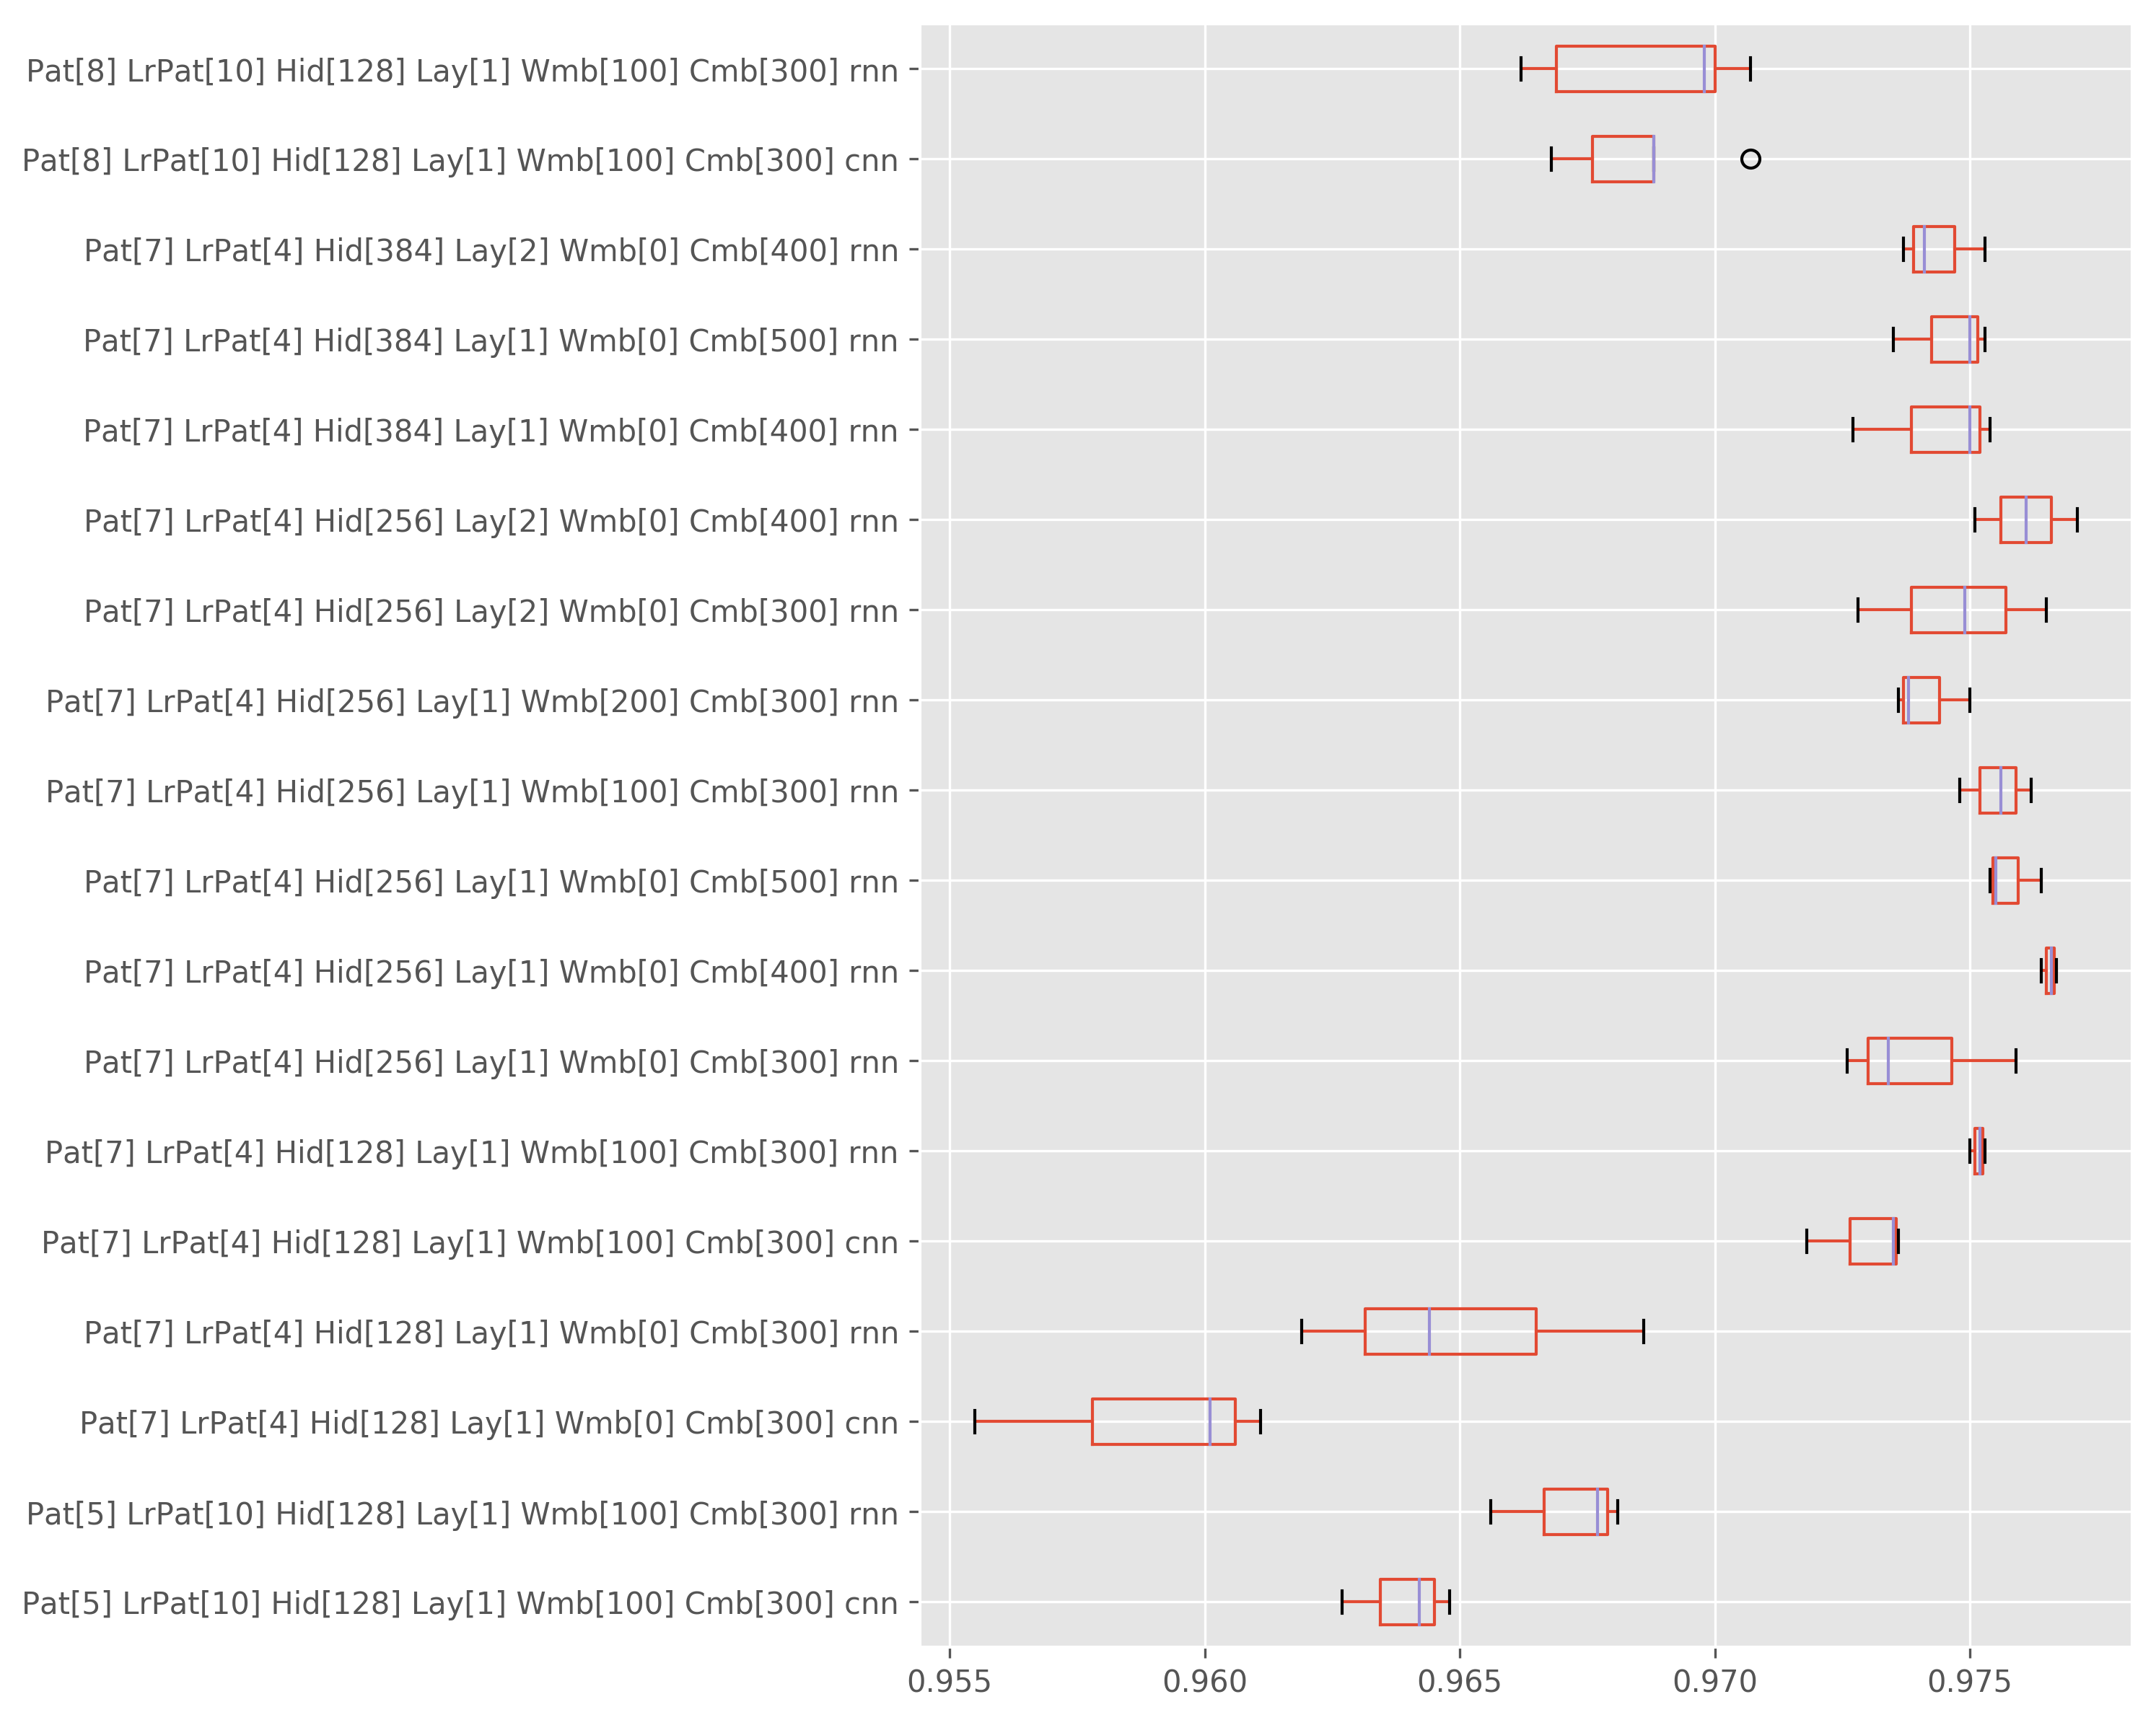
\includegraphics[width=\textwidth]{figures/chap3/entrainement/StabilityBoxPlot.png}
    \caption{Variance des résultats par configuration manuelle essayée lors de la recherche manuelle d'optimisation.}
    \label{fig:training_variation_per_model}
\end{figure}